\documentclass[12pt]{article}

\usepackage[utf8]{inputenc}
\usepackage[T1]{fontenc}  
\usepackage{hyperref}    
\usepackage{url}   
\usepackage{graphicx}
\usepackage{tabularx}
\usepackage{mathptmx}
\usepackage{indentfirst}
\usepackage{subfig}

\graphicspath{ {./graphics/} }

\hypersetup{
	colorlinks=true,
	linkcolor=blue,
	filecolor=magenta,      
	urlcolor=cyan,
}
\urlstyle{same}

\newcolumntype{C}[1]{>{\centering\arraybackslash}p{#1}}
\newcommand{\comment}[1]{}


\title{\textbf{File transfer - Sliding window protocol}}

\author{
 	Echipa: 6
	\\
	Beldiman Vladislav \\ Grupa 1305A
	\\
	Hârțan Mihai-Silviu \\ Grupa 1305B
	\\
	Timofti Gabriel \\ Grupa 1305B
}

\begin{document}

\noindent\begin{minipage}{0.1\textwidth}
	
\includegraphics[width=1.1cm]{logo_AC.png}
\end{minipage}
\hfill
\begin{minipage}{1\textwidth}\raggedright
	Universitatea Tehnică "Gheorghe Asachi" din Iași\\
	Facultatea de Automatică și Calculatoare\\
	Prelucrarea Imaginilor - Proiect
\end{minipage}

\vspace{5cm}
{\let\newpage\relax\maketitle}
\newpage

\tableofcontents
\newpage

\section{Introduction}

Sliding window protocols are used for reliable in-order delivery of packets is required, such as in the Transmission Control Protocol (TCP). They are also used to improve efficiency when the channel may include high latency. Our application goal is to reliably transfer a file over UDP using the Go-Back-N algorithm.

\section{Algorithms}

\subsection{Sliding window protocol}

\bigskip
\textbf{The Sliding Window Algorithm}
\bigskip

According to [1] the sliding window algorithm works as follows:

First, the sender assigns a sequence number, denoted \textbf{SeqNum}, to each frame. The sender maintains three variables: The send window size, denoted \textbf{SWS}, gives the upperbound on the number of outstanding (unacknowledged) frames that the sender can transmit; \textbf{LAR} denotes the sequence number of the last acknowledgment received; and \textbf{LFS} denotes the sequence number of the last frame sent. The sender also maintains the following invariant: LFS - LAR $\leq$ SWS.

When an acknowledgment arrives, the sender moves LAR to the right, thereby allowing the sender to transmit another frame. Also, the sender associates a timer with each frame it transmits, and it retransmits the frame should the timer expire before an ACK is received.

The receiver maintains the following three variables: The receive window size, denoted \textbf{RWS}, gives the upper bound on the number of out-of-order frames that the receiver is willing to accept; \textbf{LAF} denotes the sequence number of the largest acceptable frame; and \textbf{LFR} denotes the sequence number of the last frame received. The receiver also maintains the following invariant: LAF - LFR $\leq$ RWS.

When a frame with sequence number SeqNum arrives, the receiver takes the following action. If SeqNum $\leq$ LFR or SeqNum > LAF, then the frame is outside the receiver's window and it is discarded. If LFR < SeqNum $\leq$ LAF, then the frame is within the receiver's window and it is accepted. Now the receiver needs to decide whether or not to send an ACK. Let \textbf{SeqNumToAck} denote the largest sequence number not yet acknowledged, such that all frames with sequence numbers less than or equal to SeqNumToAck have been received. The receiver acknowledges the receipt of SeqNumToAck, even if higher numbered packets have been received. This acknowledgment is said to be cumulative. It then sets LFR = SeqNumToAck and adjusts LAF = LFR + RWS.

\textit{The same notations as in [1] will be used in further sections. In addition, \textbf{MaxSeqNum} will denote the number of available sequence numbers, and \textbf{NextSeqNum} will track the next packet to send.}

If the sender receives a duplicate ACK message, an untreated case in [1],  it simply ignores the message.

\subsection{Go-Back-N}

The Go-Back-N implementation of the sliding window protocol uses a SWS > 1, but has a fixed RWS = 1, thus the receiver refuses to accept any other packet but the next one in sequence. As RWS = 1, the sender only needs one timer for the entire window, and, when the timer expires it will resend the entier window. Furthermore, RWS = 1 means that MaxSeqNum $\geq$ SWS + 1 is sufficient. [1]

If a packet is lost in transit or arrives but is corrupted, all following packets are discarded until the missing packet is retransmitted which implies a minimum delay of a round-trip time and a timer timeout. Consequently, it is not efficient on connections that suffer frequent packet loss and/or from noise.

In the case that the receiver is sent a duplicate packet, it sends an ACK message of SeqNumToAck - 1.

%\subsection{Selective Repeat}
%https://techdifferences.com/difference-between-go-back-n-and-selective-repeat-protocol.html
% Furthermore, RWS = SWS means that SWS < (MaxSeqNum + 1) \ 2 is sufficient. [1]

\newpage
\subsection{Block diagrams}

\begin{figure}[h!]
	\caption{Block diagram of Go-Back-N algorithm. \href{http://www.myreadingroom.co.in/notes-and-studymaterial/68-dcn/813-go-back-n-arq-protocol.html}{[Source]}}
	\centering
	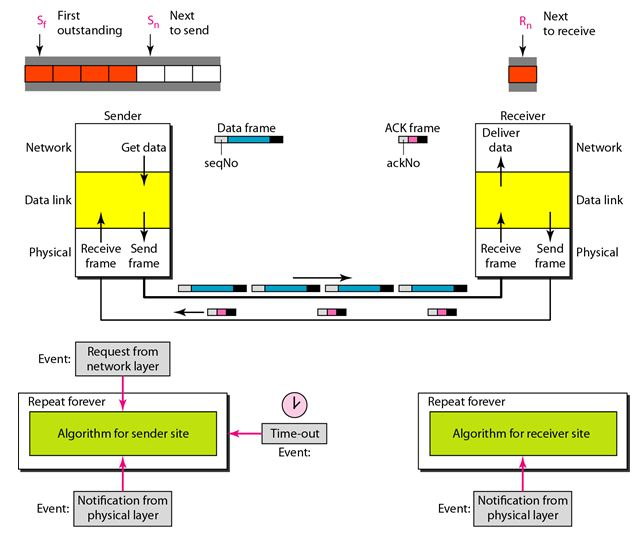
\includegraphics[width=\linewidth]{gbn.jpg}
	\label{fig:fig1}
\end{figure}

\subsection{Components}

\subsubsection{Sender}

TODO

\subsubsection{Receiver}

TODO

\subsubsection{Timer}

TODO

\subsubsection{Logger}

TODO

\subsubsection{Window}

TODO

\subsubsection{Sender Packet Handler}

TODO

\subsubsection{Reciever Packet Handler}

TODO

\subsubsection{Sender Acknowledgement Handler}

TODO

\subsubsection{Reciever Acknowledgement Handler}

TODO

\section{Git repository}

\url{https://github.com/gabitim/RC_Proiect}

\section{Reference}

\small

[1] Peterson L. L. and Davie B. S. Computer Networks a systems approach. (Fifth edition)

\end{document}